\chapter{基于国产AI处理器的Top-k算法测试验证}

本章首先介绍了Topk-k算子测试用到的实验环境,同时也描述了整个算子测试的流程。
接着自行编写脚本生成大量的测试用例,用于测试自实现 Top-k 算子的准确度是否满足要求,
以确认功能是否正确。
然后测试了不同输入规模下,Topk 算子相对于全排序Top-k算子 和 Nvidia芯片上Top-k算子的性能表现情况。
最后将自实现
 Top-k 算子集成在Pytorch深度学习框架中,对目前比较流行的模型进行训练,
 并通过检测结果验证了Top-k 算子的可用性。

\section{实验环境与测试流程}
\subsection{实验环境}

测试的环境配置如表~\ref{tab:peizhi}所示。
\begin{table}[h]
    \centering
    \caption{硬件环境配置}
    \begin{tabular}{|l|l|}
    \hline
    类型 & 配置信息 \\
    \hline
    AI处理器 & DLP-M处理器 \\
    \hline
    CPU & Intel Xeon Silver 4114 \\
    \hline
    Nvidia GPU & A100-40G \\
    \hline
    操作系统 & CentOS - 7 \\
    \hline
    开发语言 & BC 4.7.0, C++11, Python 2.7.5 \\
    \hline
    编译器 & CC 4.7.1, gcc 4.8.5 \\
    \hline
    \end{tabular}
    \label{tab:peizhi}
    \end{table}
    
    本次实验以 CPU+国产AI 处理器(以下简称 MLU)异构编程模式进行,用到了BC、C++ 以及 Python 
    三种编程语言。BC 编程语言用于实现 MLU 端的 Top-k 算法计算过程;
    C++ 编程语言则用于实现 CPU 端的数据准备;
    Python 编程语言用于 编写测例用例生成脚本。
    CC(Compiler Collection,BC 语言编译器)是基于 Clang和 LLVM 开发的 BC 编译器主驱动程序
    ,负责将 BC 源码文件编译为 MLISA 汇编文件。
    

\subsection{测试流程}
\begin{enumerate}
    \item 通过 RT 接口初始化设备,RT 包含设备管理、内存管理、任务队列管理、 设备端程序执行、通知管理等功能,使用 BC 编写的程序需要借助于 RT 提供的 接口才能运行在 MLU 设备上。
    \item 初始化 Top-k 描述符,并为保存 Top-k 参数内容的结构体创建一个句柄。 同时计算出当前输入参数下计算得到的 Top-k 特征向量需要占用的内存空间大 小, 并分配对应的内存空间。
    \item 准备输入数据,调用 RT 接口分配设备内存,并将输入数据拷贝到设备 内存中。
    \item MLU 端调用自实现的 Top 算子,得到 Top-看 特征向量。CPU 端调用 RT接口等待任务队列执行完成。
    
    \item 调用RT接口将Top-k算子的计算结果复制到主机侧。
    \item 主机侧调用Top-k的串行实现,得到比对的计算结果。
    \item 将设备端的计算结果与主机端的计算结果进行比较。
    \item 调用RT接口,释放主机端和设备端的内存以及任务队列等资源。
    
\end{enumerate}
整个计算流程如图~\ref{fig:test}所示:

\begin{figure}[ht]
    \centering
    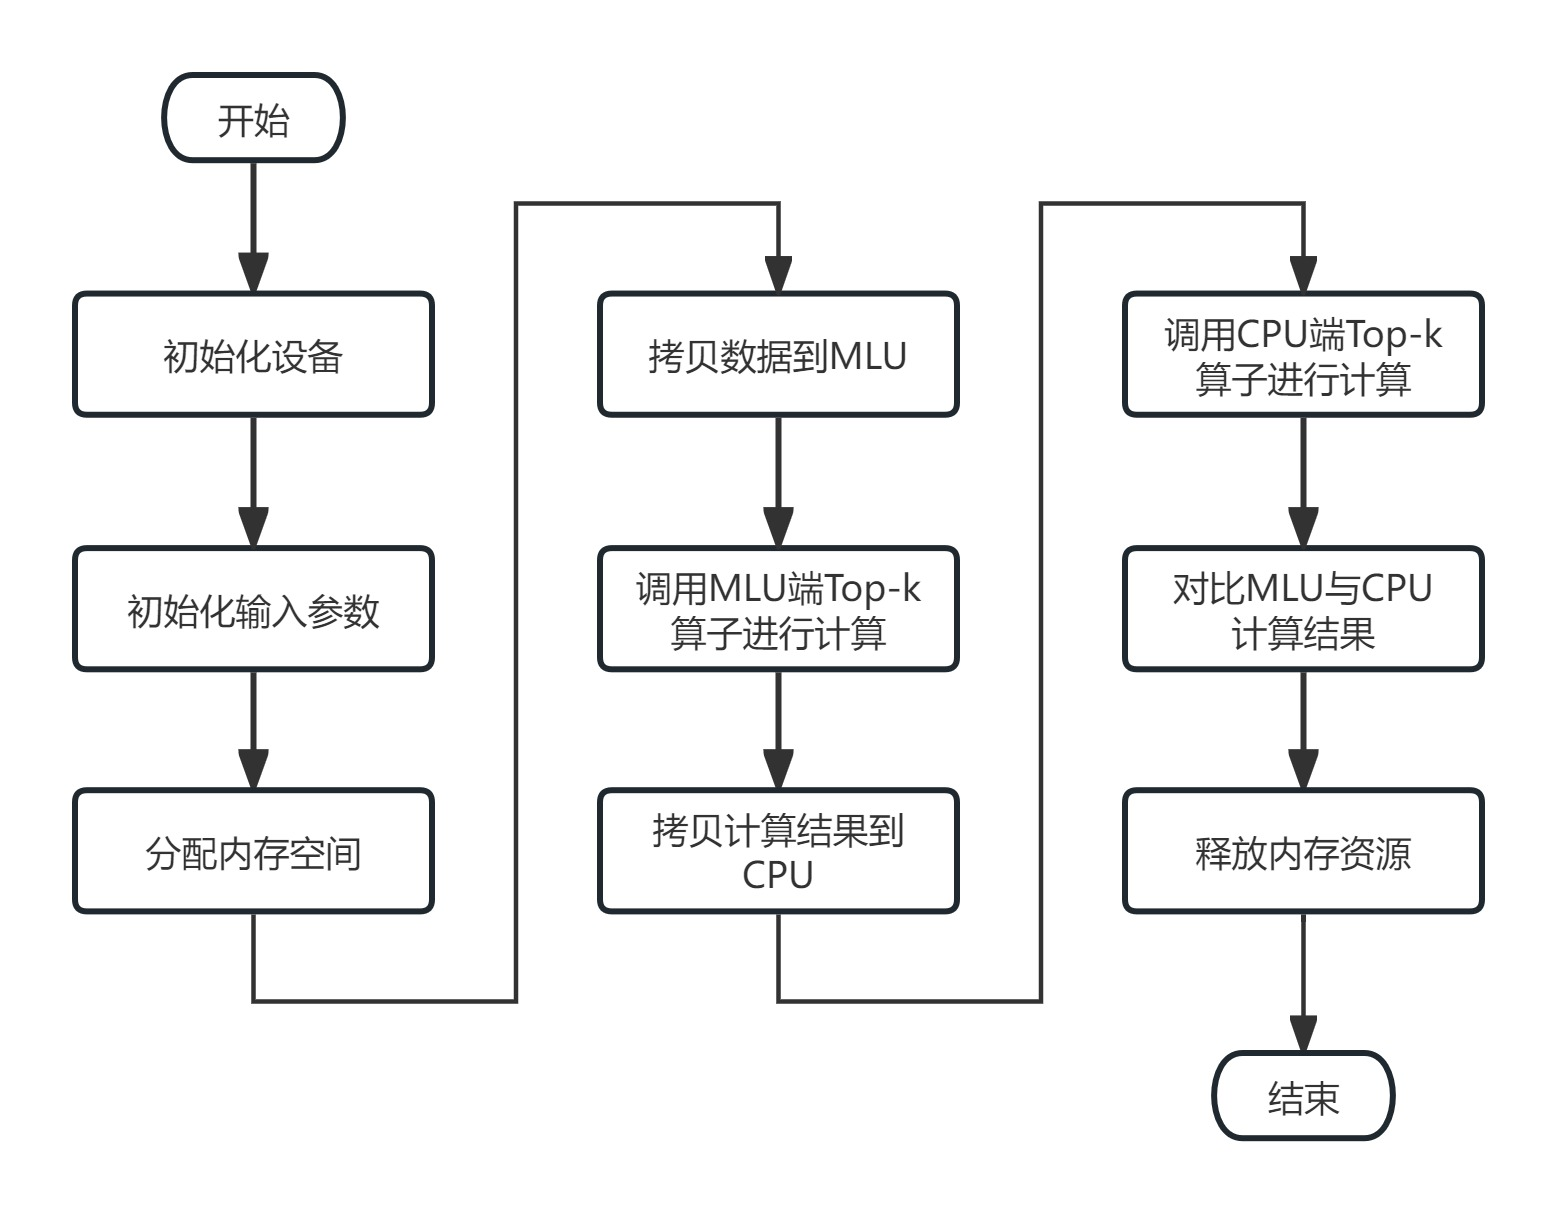
\includegraphics[width=0.85\textwidth]{test_1.jpg}
    \caption{RadixSelect测试流程图}
    \label{fig:test}
    % \note{注:图注的内容不宜放到图题中。}
\end{figure}


\section{Top-k算子功能测试}
在完成深度学习处理器的Top - K算子实现后,便可以开展算子的功能性与性能验证工作。
首先是功能验证,其主要内容如下:
\begin{enumerate}
\item 对不同维度(dim)下Top-k查询结果的正确性进行验证。
\item 针对不同k值下的查询结果正确性进行验证。
\item 检验经largest排序后的数据返回是否正确。
\end{enumerate}

在进行Top-k正确性验证时,将计算结果与CPU计算结果进行对比,
误差计算公式见,其总mlu\_output表示设备端的计算结果,cpu\_output表示主机端使用CPU的计算结果。
    \begin{equation}
    \label{eq:diff1}
    diff1 = \frac{\sum \vert baseline - mlu \vert}{\sum \vert baseline \vert + \epsilon}
    \end{equation}
    
    \begin{equation}
    \label{eq:diff2}
    diff2 = \frac{\sum (baseline - mlu)^2}{\sum (baseline)^2 + \epsilon}
    \end{equation}
其中,diff1表示与CPU返回的Top-k计算结果的相对误差,
diff2表示与CPU返回的Top-k数据的均方差。
考虑到Top-k算子仅仅只是筛选类算子,不在原数据上做具体的操作。因此diff1和diff2应当为0才能满足精度要求。
由于Top-k算子需要输出具体的值和坐标(index),因此以下的精度表格中,
diff1 = diff1\_value + diff1\_index,
diff2 = diff2\_value + diff2\_index。
本部分主要展示输入数据的数据类型为float和int的误差。小k场景下的Top-k算子的精度测试结果
如表~\ref{ab:presicionsmallk}所示。
\begin{table}
\centering
\caption{小k场景下Top-k功能测试表}
\label{tab:presicionsmallk}
\begin{tabular}{clllll}
    \toprule
    数据规模      &dim   & k  & largest & diff1    & diff2 \\
    \midrule
    (10000) int &0  & 100      & True      & 0.000000 & 0.000000 \\
    (1024,3000000)int&1 & 8000 & False      & 0.000000 & 0.000000 \\
    (1,1000000,4,2)int &1  & 5000 & True      & 0.000000 & 0.000000 \\
    (1,1000,4,2)int &1  & 500 & False      & 0.000000 & 0.000000 \\
    
    (1024,3,300,4,8)float&2 & 300 & False      & 0.000000 & 0.000000 \\
    (100, 3, 30000, 4, 10240000)float&4 & 20 & True      & 0.000000 & 0.000000 \\
    (1,1,1,10240000)float & 3 & 8192 & False      & 0.000000 & 0.000000 \\
    (1,1000,10)float & 1  & 500 & True      & 0.000000 & 0.000000 \\
    
\bottomrule
\end{tabular}
\end{table}
片上内存空间大小主要针对NRAM内存大小,结合具体实现过程,将不小于10000的k值视为大k场景。其精度测试结果见
表~\ref{tab:presicionbigk}。由测试结果可以看出,基于RadixSelect算法实现的Top-k算子,分别在大/小k场景下,皆满足对应参数下的
精度要求,与CPU计算输出结果的各误差均为0\%。
\begin{table}
    \centering
    \caption{大k场景下Top-k功能测试表}
    \label{tab:presicionbigk}
    \begin{tabular}{clllll}
        \toprule
        数据规模       &dim  & k  & largest & diff1    & diff2 \\
        \midrule
        (102400) int&0&  12000     & True      & 0.000000 & 0.000000 \\
        (1024,3000000)int&0 & 10000 & False      & 0.000000 & 0.000000 \\
        (100, 3, 30000, 4, 8)int&2 & 15000 & True      & 0.000000 & 0.000000 \\
        (400, 2000000)int&1 & 15000 & False      & 0.000000 & 0.000000 \\
        
        (1,1,1,10240000)float &3& 1000000 & False      & 0.000000 & 0.000000 \\
        (1,1000000,4,2)float  &1 & 20000 & True      & 0.000000 & 0.000000 \\
        (1,1,1,10240000)float&3 & 1000000 & False      & 0.000000 & 0.000000 \\
        (200,33669)float&1 & 14931 & True      & 0.000000 & 0.000000 \\
    
    \bottomrule
    \end{tabular}
    \end{table}

\section{Top-k算子性能测试}
在本节中,我们针对两种场景下的核函数进行性能测试。首先是对比优化前后的性能提升效果。
而后分别与DLP-M原版本 Top-k 算子,Nvidia-A100 Top-k 算子显卡进行性能对比。
\subsection{小k场景下RadixSelect算子性能测试}
\paragraph{优化前后性能对比}
在使用前文中的各种优化手段后,本节对(100, 1310720)这一数据规模进行了实验测试,
以说明对于任务规模优化,I/O优化,计算效率优化后的加速效果。
具体数据如表~\ref{tab:bench_littlek_upgrade}所示。
在经过优化之后,性能加速效果维持在48\%左右。

\begin{table}
    \centering
    \caption{小k场景优化前后测试表}
    \label{tab:bench_littlek_upgrade}
    \begin{tabular}{cllllll}
        \toprule
        数据规模       &k  & dim  & largest & 优化前耗时(us)    & 优化后耗时(us) &加速比\\
        \midrule
        (100,1310720) float&16&  1     & True      & 5970.96 & 3042 &  0.4905\\
        (100,1310720) float&32&  1     & True      & 5988.87 & 3050 &  0.4907\\
        (100,1310720) float&50&  1     & True      & 6168.98 & 3200 &  0.4813 \\
        (100,1310720) float&75&  1     & True      & 6185.77 & 3211 &  0.4809 \\
        (100,1310720) float&100&  1     & True      & 6162.35& 3187 &  0.4828 \\
        (100,1310720) float&1000&  1     & True      & 6727.01 & 3493 & 0.4807 \\
        (100,1310720) float&8192&  1     & True      & 13016.7 & 6859 & 0.4731 \\
        
        \bottomrule
    \end{tabular}
    \end{table}
具体效果如图{zhexian-lk-upgrade.png}所示,
对比效果图我们可以发现,在相同输入规模下,随着k的增加,优化前后的时间都在逐渐增加。
这反映了对于相同的输入规模而言,k的值越大,单个MLU-Core的任务量也就越大,在执行RadixSelect
算法时,其“FIND TARGET BUCKET”与”FILTER“中的任务也将更复杂。

\begin{figure}[ht]
        \centering
        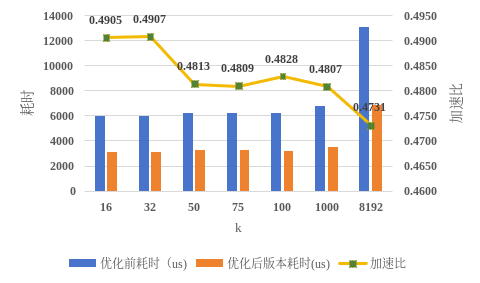
\includegraphics[width=0.8\textwidth]{zhexian-lk-upgrade_1.png}
        \caption{小k场景优化前后对比图}
        \label{fig:bench_littlek_upgrade_zhexian}
        % \note{注:图注的内容不宜放到图题中。}
    \end{figure}
    

\paragraph{与原版本性能对比}
原版本小k场景下的Top-k算子主要使用的是基于冒泡排序的Top-k算子,其串行算法的时间复杂度为O(kN)。
在k和N都不太大的时候,其性能表现尚可,但是当数据规模较大时,Top-k算子的性能将会受到影响。
同时,当数据中存在Nan和Inf时,原版本实现为了满足与CPU结果对齐的要求,将会引入
很多对于正常数据而言不必要的操作,性能将会大幅度下降。此时Top-k算子主要基于RadixSort全排序算法。
其性能对比数据如表~\ref{tab:bench_littlek}所示。可以发现小k场景下的实现明显优于原版本。
\begin{table}
    \centering
    \caption{小k场景与原版本性能对比表}
    \label{tab:bench_littlek}
    \begin{tabular}{cllllll}
        \toprule
        数据规模       &k  & dim  & largest & RadixSelect耗时    & 原版本耗时 &加速比\\
        \midrule
        (1,80000) float&100&  1     & True      & 14.99 & 78.22 & 0.8093\\
        %(1,391680) float&1000&  1     & True      & 79 & 10917  & 0.9721 \\  

        (16,136960) float&10000&  1     & True      & 280 & 1535 & 0.8176\\
        (32,136960) float&10000&  1     & True      & 400 & 3060 & 0.8693\\
        (64,136960) float&10000&  1     & True      & 790 & 6405 & 0.8767\\
        
        (100,1310720) float&16&  1     & True      & 3042 & 2826.9 &  -0.076\\
        (100,1310720) float&32&  1     & True      &  3050& 2910.6 &  -0.048\\
        (100,1310720) float&50&  1     & True      & 3200 & 3013.2 &  -0.062 \\
        (100,1310720) float&75&  1     & True      & 3211 & 3040.2 &  -0.056 \\
        (100,1310720) float&100&  1     & True      & 3187& 3113.1 &  -0.024 \\
        (100,1310720) float&1000&  1     & True     & 3493& 3842.1 &   0.091 \\
        (100,1310720) float&8192&  1     & True      & 6859& 13170.6 & 0.479 \\
      
        % (100,1310720) float&1 &  16     & True      & 790 &  & 0.8767\\
        % (64,136960) float&10000&  1     & True      & 790 &  & 0.8767\\
        

        \bottomrule
    \end{tabular}
    \end{table}

将B和k分别固定为136960和10000,对于不同的A的数值进行绘图,如图~\ref{fig:bench_littlek-vsorigin}所示。
可以发现随着输入数据规模的增大,相较于原来版本的加速效果越来越好。
    \begin{figure}[ht]
        \centering
        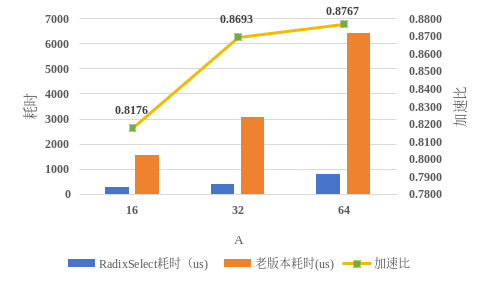
\includegraphics[width=0.65\textwidth]{zhexian-lk-vsorigin_1.png}
        \caption{与原版本性能对比图}
        \label{fig:bench_littlek-vsorigin}
        % \note{注:图注的内容不宜放到图题中。}
    \end{figure}
    

    \begin{figure}[ht]
        \centering
        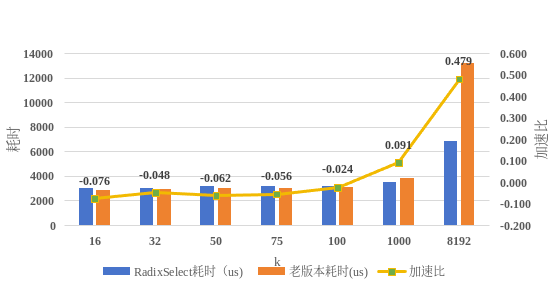
\includegraphics[width=0.65\textwidth]{zhexian-lk-vsorigin_2.png}
        \caption{与原版本性能对比图}
        \label{fig:bench_littlek-vsorigin_1}
        % \note{注:图注的内容不宜放到图题中。}
    \end{figure}
    

\paragraph{与A100-GPU性能对比}
小k场景下RadixSelect算子性能与NVIDIA A100 GPU进行性能对比,其性能测试数据如表
~\ref{tab:lkvsa100}所示。
\begin{table}
    \centering
    \caption{小k场景下DLP-M/A100性能对比表}
    \begin{tabular}{cllll}
    \toprule
    数据规模 & k &   DLP-M耗时(us) & A100耗时(us) & 加速比 \\
    \midrule
    (1,16384) & 1024    & 25 & 105 & 0.76 \\
    (1,16384) & 2048   & 23 & 115 & 0.80 \\
    (1,16384) & 4096   & 31 & 116 & 0.73 \\
    (1,16384) & 8192   & 35 & 180 & 0.81 \\
    (1,65536) & 1024    & 40 & 72 & 0.44 \\
    (1,65536) & 2048    & 46 & 75 & 0.39 \\
    (1,65536) & 4096    & 56 & 76 & 0.26 \\
    (1,65536) & 8192   & 74 & 138 & 0.46 \\

    (1,131072) & 1024    & 45 & 79 & 0.43 \\
    (1,131072) & 2048    & 51 & 80 & 0.36 \\
    (1,131072) & 4096    & 67 & 82 & 0.18 \\
    (1,131072) & 8192   & 102 & 145 & 0.30 \\
    

    (100,1310720) &16      & 3042 & 3019.5 &  -0.01\\
    (100,1310720) &32 &  3050& 3046.1 &  0.00\\
    (100,1310720) &50  & 3200 & 3043.4 &  -0.05 \\
    (100,1310720) &75   & 3211 & 3036.4 &  -0.06 \\
    (100,1310720) &100    & 3187& 3042.9 &  -0.05 \\
    (100,1310720) &1000   & 3493& 3074   &   -0.14 \\
    (100,1310720) &8192    & 6859& 3322.9 & -1.06 \\

    \bottomrule
    \end{tabular}
\label{tab:lkvsa100}    
\end{table}
    
    在相同输入规模,不同k值下进行绘图,如图~\ref{fig:bench_littlek_vsa100_zhexian}
    和~\ref{fig:bench_littlek_vsa100_2_zhexian}所示。随着输入规模的增大,
    DLP-M平台与A100平台上的Topk算子的耗时都逐步增加,并且随着数据规模的增大,加速比总体上呈现
    逐步下降的趋势,当k过大时(如8192),DLP-M的加速比骤然变大,这应当主要由于
    DLP-M与A100的体系结构差异导致的,即此时A100上的Top-k算子可能切换到了别的版本实现中,但由于时间问题,并没有进一步深究。
    整体而言,在输入较小时,相较于A100可以达到3.5-4倍的提速。
    在输入较大时,相较于A100可以达到1.3-1.8倍的提速。

    \begin{figure}[ht]
        \centering
        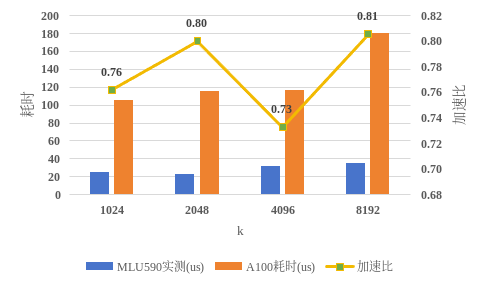
\includegraphics[width=0.75\textwidth]{zhexian-lkvsA100-11.png}
        % \caption{小k场景优化前后对比图}
        \label{fig:bench_littlek_vsa100_zhexian}
        % \note{注:图注的内容不宜放到图题中。}
    \end{figure}
    
    \begin{figure}[ht]
        \centering
        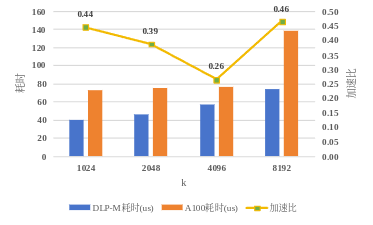
\includegraphics[width=0.75\textwidth]{zhexian-lkvsA100-22.png}
        \caption{小k场景下DLP-M/A100性能对比图}
        \label{fig:bench_littlek_vsa100_2_zhexian_1}
        % \note{注:图注的内容不宜放到图题中。}
    \end{figure}
    
    \begin{figure}[ht]
        \centering
        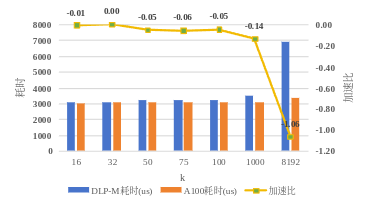
\includegraphics[width=0.75\textwidth]{zhexian-lkvsA100-3.png}
        \caption{小k场景下DLP-M/A100性能对比图}
        \label{fig:bench_littlek_vsa100_2_zhexian}
        % \note{注:图注的内容不宜放到图题中。}
    \end{figure}
    

\subsection{大k场景下RadixSelect算子性能测试}

\paragraph{优化前后性能对比}
通过对大k场景下的RadixSelect算子实现进行优化后,其在部分测试样例上的表现如表所示。
在对于(100,1310720)这一输入规模下,随着k的增大耗时逐渐增加。
相较于优化前,加速比维持在0.13-0.18之间。
\begin{table}
    \centering
    \caption{大k场景优化前后性能对比表}
    \label{tab:bench_bigk_upgrade}
    \begin{tabular}{cllllll}
        \toprule
        数据规模       &k  & dim  & largest & 优化前耗时    & 优化后耗时 &加速比\\
        \midrule
        (100,1310720) float&16384&  1     & True      & 5222 & 4453 & 0.1473\\
        (100,1310720) float&32768&  1     & True      & 6128 & 5283 & 0.1379\\
        (100,1310720) float&65536&  1     & True      & 7299 & 6279 & 0.1397\\
        (100,1310720) float&131072&  1     & True      & 8540 & 7061 & 0.1732\\
        
        
        \bottomrule
    \end{tabular}
    \end{table}
    
    
    \begin{figure}[ht]
        \centering
        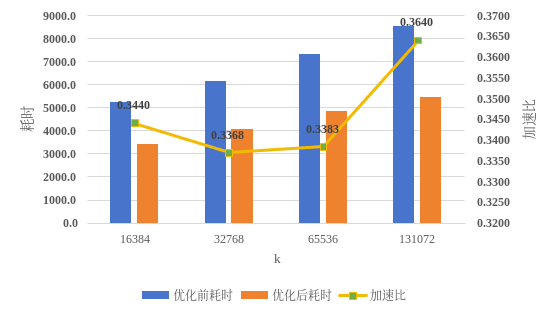
\includegraphics[width=0.8\textwidth]{zhexian-bk-upgrade-1.png}
        \caption{大k场景优化前后对比图}
        \label{fig:bench_bk_upgrade_zhexian}
        % \note{注:图注的内容不宜放到图题中。}
    \end{figure}
    



\paragraph{与原版本性能对比}
在大k场景下,大k版本的Top-k算子主要使用全排序版本,仅在最后输出时,将符合要求的k个数复制到
主机端,因此原来版本的耗时比较稳定,而对于RadixSelect而言,随着k的值越来越大,每个ML
U-Core的任务量也越来越大,在执行RadixSelect的耗时逐步增加,因此其加速比逐渐降低,
其测试数据如表~\ref{tab:bench_bigk}所示,
折线图如图~\ref{fig:bench_bk_vsorigin_zhexian}所示。
\begin{table}
    \centering
    \caption{大k场景与原版本性能对比表}
    \label{tab:bench_bigk}
    \begin{tabular}{cllllll}
        \toprule
        数据规模       &k  & dim  & largest & RadixSelect耗时    & 原版本耗时&加速比 \\
        \midrule
        (100,1310720) float&16384&  1     & True      & 3425.38 & 33832.4 & 0.8988 \\
        (100,1310720) float&32768&  1     & True      & 4063.85 & 34012.9 & 0.8805\\
        (100,1310720) float&65536&  1     & True      & 4830.00 & 34171.8 &0.8587\\
        (100,1310720) float&131072&  1     & True      & 5431.54 & 34197 & 0.8412 \\
        
        \bottomrule
    \end{tabular}
    \end{table}
    \begin{figure}[ht]
        \centering
        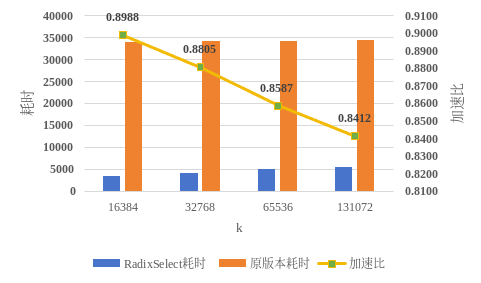
\includegraphics[width=0.7\textwidth]{zhexian-bk-vsorigin-1.png}
        \caption{与原版本性能对比图}
        \label{fig:bench_bk_vsorigin_zhexian}
        % \note{注:图注的内容不宜放到图题中。}
    \end{figure}
    
    


\paragraph{与A100-GPU性能对比}
大k场景下RadixSelect算子性能与NVIDIA A100 GPU进行性能对比,
在相同输入规模,不同k值下进行绘图,如图~\ref{fig:bench_bk_vsa100_zhexian}所示。随着输入规模的增大,
DLP-M平台与A100平台上的Topk算子的耗时都逐步增加,并且随着数据规模的增大,加速比总体上呈现
逐步下降的趋势。整体而言,相较于A100可以达到1.4-2.3倍的提速。
\begin{table}
    \centering
    \caption{大k场景下DLP-M/A100性能对比表}
    \begin{tabular}{cllll}
    \toprule
    数据规模 & k &   DLP-M耗时(us) & A100耗时(us) & 加速比 \\
    \midrule
    % (1,32768) & 16384   & 66 & 142 & 2.2 \\
    % (1,65536) & 16384    & 68.5 & 145 &  \\
    % (1,65536) & 32768   & 92.5 & 143 &  \\

    (1,131072) & 16384    & 76.2 & 153 & 0.5020\\
    (1,131072) & 32768   & 85.5 & 155 & 0.4484\\
    (1,131072) & 65536   & 102.1 & 157 & 0.3497  \\
    
    (1,262144) & 16384   & 89 & 165.3 & 0.4616  \\
    (1,262144) & 32768   & 101.2 & 167.1 & 0.3944 \\
    (1,262144) & 65536   & 121.7 & 170.1 & 0.2845 \\
    
    (100, 1310720)& 8192 & 3259.23 & 3322.9 & 0.02\\
    (100, 1310720)& 16384 & 3425.38 & 3526.3 & 0.03\\
    
    (100,1310720)&32768    & 4063.85 & 3875.4 & -0.05  \\
    (100,1310720)&65536    & 4830.00 & 4537.4 & -0.06 \\
    (100,1310720)&131072   & 5431.54 & 5789.3 & 0.06 \\
  
    \bottomrule
    \end{tabular}
    \end{table}


    % \begin{figure}[ht]
    %     \centering
    %     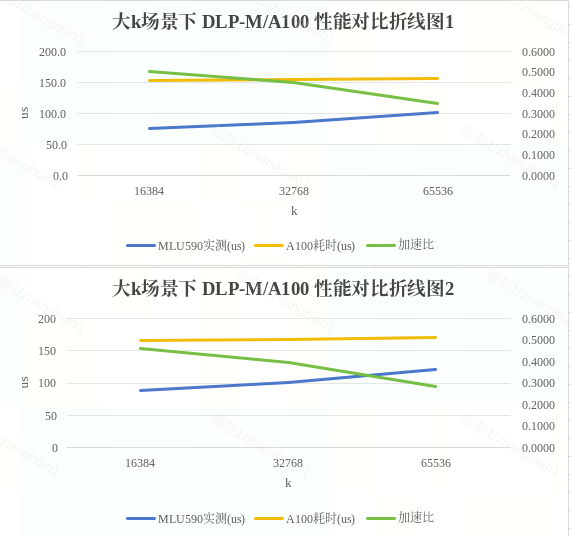
\includegraphics[width=0.7\textwidth]{zhexian-bkvsA100.png}
    %     \caption{大k场景下DLP-M/A100性能对比图}
    %     \label{fig:bench_bk_vsa100_zhexian}
    %     % \note{注:图注的内容不宜放到图题中。}
    % \end{figure}
    
    \begin{figure}[ht]
        \centering
        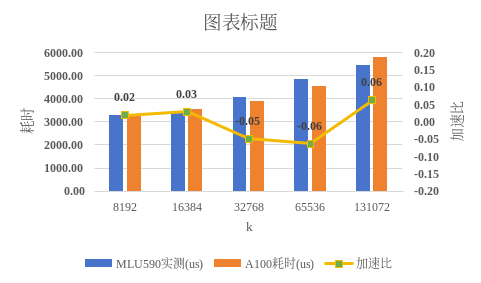
\includegraphics[width=0.7\textwidth]{zhexian-bkvsA100-1.png}
        \caption{大k场景下DLP-M/A100性能对比图}
        \label{fig:bench_bk_vsa100_zhexian_1}
        % \note{注:图注的内容不宜放到图题中。}
    \end{figure}
    

\section{Top-k算子集成测试}
Top-k算子的集成测试主要通过面向国产AI处理器的Pytorch框架进行。
它通过PyTorch社区的后端集成机制允许用户在使用原生社区PyTorch的基础上灵活、快速的接入寒武纪MLU后端。
为神经网络计算提供了强大的AI加速。


\subsection{Pytorch后端集成机制和网络搭建简介}
\paragraph{Pytorch后端集成机制}

PyTorch的后端集成核心步骤围绕着如何使新后端与框架无缝协作,主要包括注册内核、生成器、设备保护
以及元数据的序列化和反序列化等操作,确保新后端在PyTorch中能高效运行并提供完整功能。
在深度学习研究和实际应用中,针对特定硬件或自定义计算逻辑的需求日益增长。为了支持用户在不修改框
架核心代码的前提下扩展其功能,PyTorch 提供了一种灵活的扩展机制,称为 PrivateUseOne。
该机制通过注册自定义设备类型和操作逻辑,允许用户在 PyTorch 环境中实现特定需求。
PrivateUseOne 的核心功能是支持用户注册一个私有设备类型,并为其实现自定义张量操作。
例如,当需要在特殊硬件设备(如实验性芯片或 FPGA)上运行张量计算时,用户可以通过 
PrivateUseOne 定义专属的调度逻辑和运算规则。此机制基于 PyTorch 的底层设备调度框架,
使得自定义设备与原生设备类型(如 CPU、GPU)无缝集成。

实现方法包括以下几个步骤:
\begin{enumerate}
    \item {设备类型注册}用户通过调用 PyTorch 提供的接口注册自定义设备类型。
    \item{扩展张量运算}用户可以实现特定的张量操作逻辑(如加法、矩阵乘法等),并将其关联到自定义设备。
    \item{调度机制}利用 PyTorch 的调度器,将相关计算操作分发到用户定义的设备中执行。
\end{enumerate}

在MLU后端成功进行注册后,PyTorch Eager模式下算子间数据传递和存储的基本单元是tensor。
PyTorch根据tensor中的device属性值将算子分发到不同设备。
以 abs() 算子为例,在dispatch阶段会根据input\_tensor的设备属性值将算子调用分发到具体设备,
如下图所示。

\begin{figure}
    \centering
    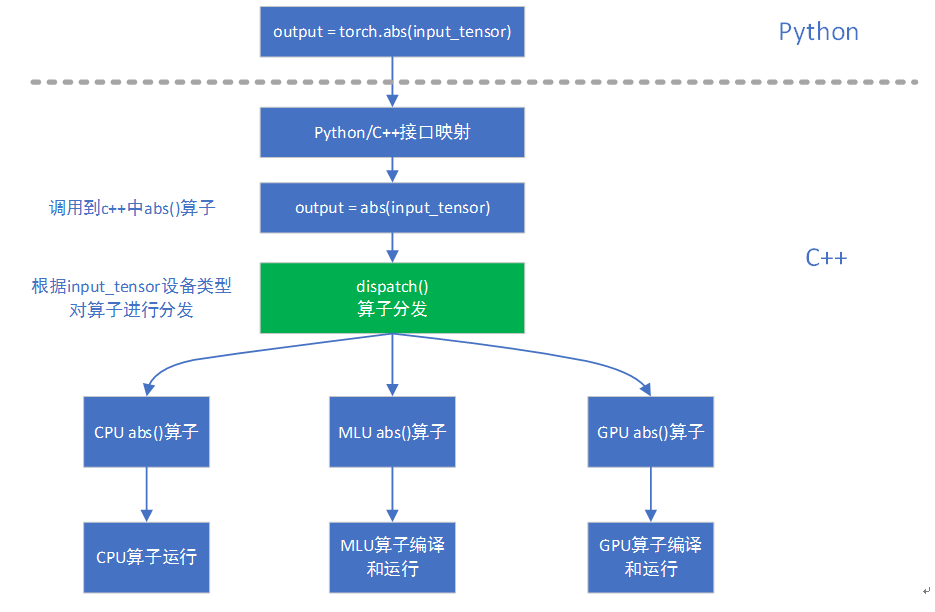
\includegraphics[width=0.8\textwidth]{mlu_operators.png}
    \caption{算子分发机制图}
    \label{fig:mlu_operators}
    % \note{注:图注的内容不宜放到图题中。}
\end{figure}

而在算子调用分发到具体设备之前,需要进行算子注册。
其基本流程如下:
算子注册的基本步骤如下:
\begin{enumerate}
    \item {定义算子接口}:
    使用 PyTorch 提供的 \texttt{native\_functions.yaml} 文件定义算子的接口及其功能。在该文件中明确指定算子的名称、输入输出参数以及调度规则。
    
    \item {实现算子功能}:
    在 C++ 或其他语言中实现算子的实际计算逻辑。对于 MLU 硬件,可以基于 Cambricon SDK 提供的算子库进行开发。
    
    \item {绑定算子与调度逻辑}:
    使用 PyTorch 的 \texttt{RegisterDispatchKey} 机制,将自定义算子绑定到 MLU 的计算后端。这一过程需要将算子注册到相应的 Backend(如 \texttt{MLU})。
    
    \item {测试算子功能}:
    编写测试用例验证算子的正确性,并使用 PyTorch 提供的单元测试框架进行全面测试,以确保算子在不同输入条件下的性能和正确性。
\end{enumerate}
其注册的关键点如下:
\begin{itemize}
    \item {文件结构}:
    修改 \texttt{native\_functions.yaml} 和相关 C++ 文件是算子注册的核心工作,不同后端(如 CPU、CUDA、MLU)需要明确区分。
    
    \item {设备适配}:
    结合 {Cambricon SDK},针对 MLU 硬件优化算子的性能,支持异构计算场景(如多设备调度)。
    
    \item {调度与调用}:
    注册后,PyTorch 会根据输入张量的设备类型,自动调用对应的算子实现。
\end{itemize}

通过以上步骤,我们可以将RadixSelect Top-k算子集成到Pytorch中,并在国产AI处理器上进行Top-k计算,供上游的模型进行使用。



\subsection{多卡训练}

% PyTorch 是一种灵活且高效的深度学习框架,广泛应用于神经网络模型的研究与开发。其动态计算图和模块化设计使得模型的搭建和训练变得直观且高效。以下从流程的角度总结了基于 PyTorch 搭建模型的主要步骤。


% \paragraph{\textbf{定义模型结构}}
% PyTorch 使用 \texttt{torch.nn.Module} 类来构建神经网络模型。用户可以通过继承该类并重写其 \texttt{forward} 方法来定义自定义模型结构。
% \begin{enumerate}
%     \item {初始化模型参数}:在 \texttt{\_\_init\_\_} 方法中定义网络的基本结构,例如卷积层、全连接层和激活函数。
%     \item {定义前向传播}:通过重载 \texttt{forward} 方法实现模型的前向传播逻辑。
% \end{enumerate}

% \paragraph {\textbf{选择损失函数与优化器}}
% 损失函数是模型优化的目标,优化器则用于更新模型参数。
% \begin{enumerate}
%     \item PyTorch 提供了多种常用损失函数(如\texttt{torch.nn.MSELoss})。
%     \item 通过 \texttt{torch.optim} 模块定义优化器(如 \texttt{SGD}、\texttt{Adam}),并设置学习率等超参数。
% \end{enumerate}

% \paragraph{\textbf{模型训练}}
% 模型训练是优化参数以最小化损失函数的过程,通常包括多个迭代周期(epochs)。
% \begin{enumerate}
%     \item {前向传播}:将数据输入模型并计算预测值。
%     \item {计算损失}:通过损失函数计算预测值与真实值之间的差异。
%     \item {反向传播}:通过 \texttt{loss.backward()} 计算梯度。
%     \item {参数更新}:利用优化器(如 \texttt{optimizer.step()})更新模型参数。
% \end{enumerate}

% \paragraph{\textbf{模型验证与测试}}
% 在训练完成后,需要使用验证集或测试集评估模型的性能。通常通过以下方式实现:
% \begin{enumerate}
%     \item 切换模型到评估模式(使用 \texttt{model.eval()})。
%     \item 禁用梯度计算(通过 \texttt{torch.no\_grad()})。
%     \item 评估模型在测试集上的指标(如准确率、精确率等)。
% \end{enumerate}


% 上述流程体现了 PyTorch 在深度学习模型开发中的高灵活性和模块化特性。通过合理组织代码结构,
% 我们可以快速高效的完成从数据预处理、模型定义到训练与验证的完整流程,
% 从而专注于模型性能的优化和创新性算法的探索。

Cambricon PyTorch (CATCH)目前支持对tensor进行单机多卡和多机多卡的卡间集合通信,对网络进行单机多卡和多机多卡的分布式训练。
目前支持以下通信原语:卡间广播(broadcast)、卡间规约(allreduce、reduce、reduce\_scatter)、
卡间收集(allgather、all-to-all),支持进程间同步(barrier)。
其中,卡间规约又包含4种操作:求和、求连乘、求最大值、求最小值。
原生框架的Distributed Data Parallel分布式训练机制在单个机器上有两种使用模式:
a、单进程多卡;b、多进程多卡,每个进程用一张卡(官方推荐模式)。

当前阶段,MLU设备间通信依赖MLU设备通信后端CNCL(Cambricon Communications Library,寒武纪通信库)。
仅需要在初始化进程组实例时,将backend 参数变换为 cncl,
即可以基于国产AI处理器使用分布式训练框架进行分布式训练,继而进行算子的集成测试。





\subsection{模型和数据集准备}
在集成测试中,本文选用Mixtral8\times7B大模型,其主要基于 Transformer 架构,支持上下文长度达到 32k token,并且前馈块被 Mixture-of-Expert(MoE)层取代。
模型主要参数如下表~\ref{tab:model}。
\begin{table}
    \centering
    \caption{模型参数表}
    \label{tab:model}
    \begin{tabular}{cl}
        \toprule
        Parameter       &Value   \\
        \midrule
        dim & 4096 \\
        n\_layers & 32 \\
        head\_dim & 128 \\
        hidden\_dim & 14336 \\
        n\_heads & 32 \\
        n\_kv\_heads & 8 \\
        context\_len & 32768 \\
        vocab\_size & 32000 \\
        num\_experts & 8 \\
        top\_k\_experts & 2 \\
        \bottomrule
    \end{tabular}
    \end{table}

    其中,在整个模型架构中,本文所涉及的Top-k算子主要集中在MOE层。
    其主要结构如图~\ref{fig:moe}所示,
\begin{figure}[ht]
    \centering
    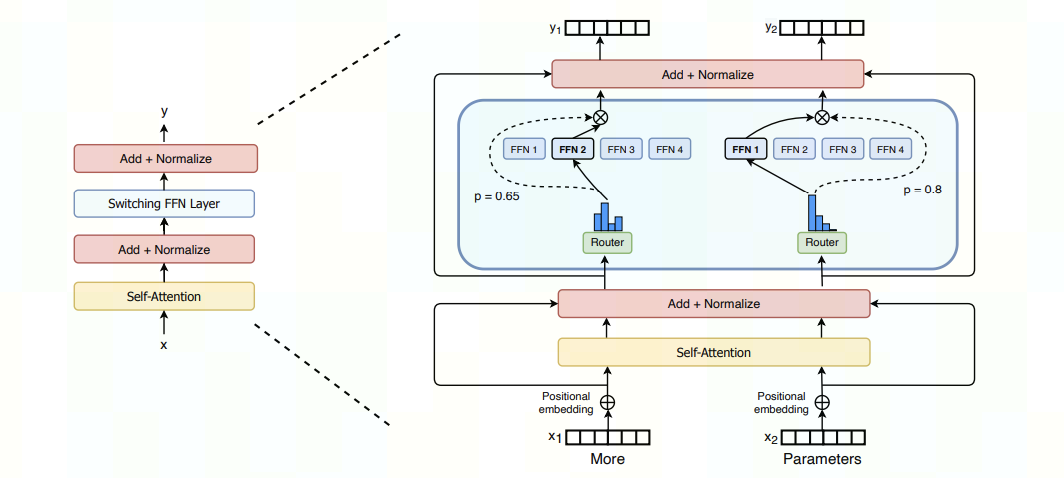
\includegraphics[width=1.0\textwidth]{moe.png}
    \caption{MOE模型结构图}
    \label{fig:moe}
    % \note{注:图注的内容不宜放到图题中。}
\end{figure}

而MOE层的模型结构主要有两个关键部分组成:
\begin{enumerate}
    \item{稀疏 MoE 层}: 这些层代替了传统 Transformer 模型中的前馈网络 (FFN) 层。MoE 层包含若干“专家”(Mixtral8\times7B 中有 8 个),每个专家本身是一个独立的神经网络。在实际应用中,这些专家通常是前馈网络 (FFN),但它们也可以是更复杂的网络结构,甚至可以是 MoE 层本身,从而形成层级式的 MoE 结构。
    \item {门控网络或路由}:
    这个部分用于决定哪些token被发送到哪个expert。例如,在下图中,“More”这个token可能被发送到第二个专家,而“Parameters”这个token被发送到第一个专家。有时,一个token甚至可以被发送到多个专家。token的路由方式是 MoE 使用中的一个关键点,因为路由器由学习的参数组成,并且与网络的其他部分一同进行预训练。
\end{enumerate}
计算过程如下述公式。
\begin{equation}
MoE(x) = \sum_{i = 1}^{n} (G(x)_i E_i(x))
\end{equation}

\begin{equation}
G(x) = TopK(\text{softmax}(W_g x + \epsilon))
\end{equation}

上述第1个公式表示了包含 $n$ 个专家的MoE层的计算过程。具体来讲,首先对样本 $x$ 进行门控计算,$W$ 表示权重矩阵;然后,由 $\text{Softmax}$ 处理后获得样本 $x$ 被分配到各个 $\text{expert}$ 的权重;然后,只取前 $k$(通常取1或者2)个最大权重;最终,整个 $\text{MoE Layer}$ 的计算结果就是选中的 $k$ 个专家网络输出的加权和。

在确定好模型之后,需要进行数据集的准备。在本集成测试实验中,使用的数据集为OpenWebText,
其是一个大规模的文本数据集,在自然语言处理(NLP)领域,特别是在无监督预训练语言模型的开发中
具有重要地位。它包含数十亿个单词,能够为语言模型提供丰富的语言信息。
它主要用于预训练语言模型,如OpenAI的 GPT(Generative Pretrained Transformer)系列模型。在预训练阶段,语言模型通过学习 OpenWebText 中的文本序列,捕捉语言的统计规律和语义信息,从而构建语言的内在表示。
在进行训练之前,需要将其转换为raw-data形式,相关命令如下:


\subsection{结果展示}
由于训练成熟的大语言模型需要大量的训练技巧和硬件资源,对于算子的集成测试而言,其是没有必要的。
因此本节中仅对比模型在国产AI芯片和NVIDIA GPU前100 step的训练表现,
以此来作为国产AI芯片上的Top-k算子可用的依据。
    
GPU与MLU模型训练loss如图~\ref{fig:loss}所示,我们可以发现,在整个训练过程中,
国产AI芯片的训练loss趋势与NVIDIA A100 GPU的loss趋势基本保持吻合。 
\begin{figure}[ht]
    \centering
    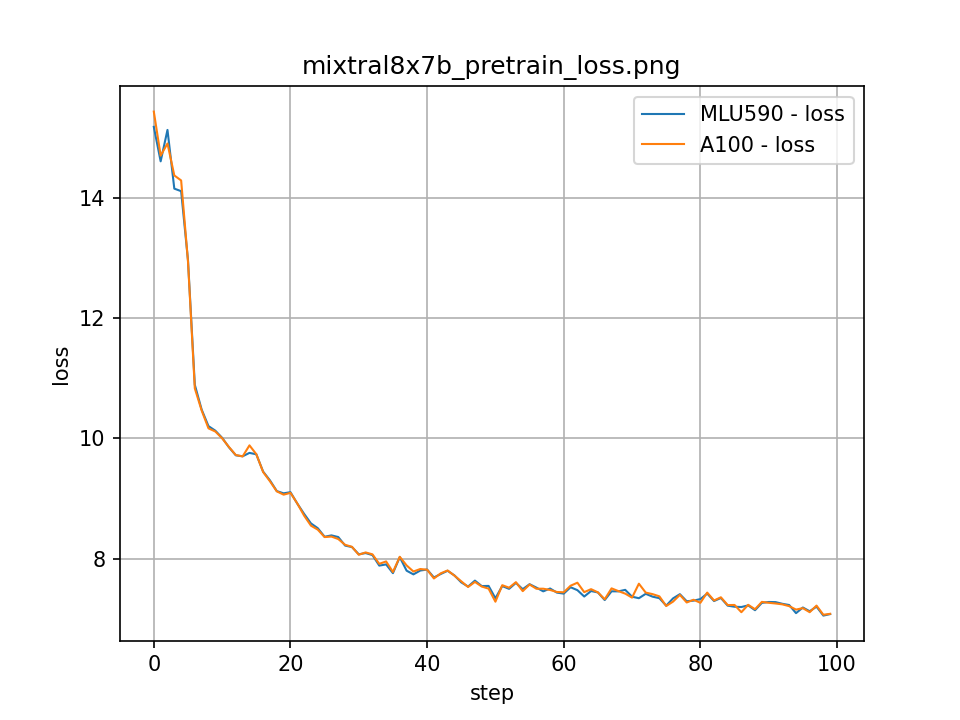
\includegraphics[width=0.6\textwidth]{loss.png}
    \caption{GPU/MLU 训练图}
    \label{fig:loss}
    % \note{注:图注的内容不宜放到图题中。}
\end{figure}
为了更好的衡量两只之间的吻合程度,我们进行相对误差分析,其公式如~\ref{eq:loss_error}所示:
\begin{equation}
    \label{eq:loss_error}
    diff = \frac{\vert mluloss - gpuloss \vert}{gpuloss}
\end{equation}
对于相对误差,一般要求其低于0.01。GPU与MLU模型训练loss相对误差如图~\ref{fig:mlu_gpu_loss_error}所示,我们可以发现,
在每个step中,相对误差基本都维持在0.01以下,满足了基本要求。
\begin{figure}[ht]
    \centering
    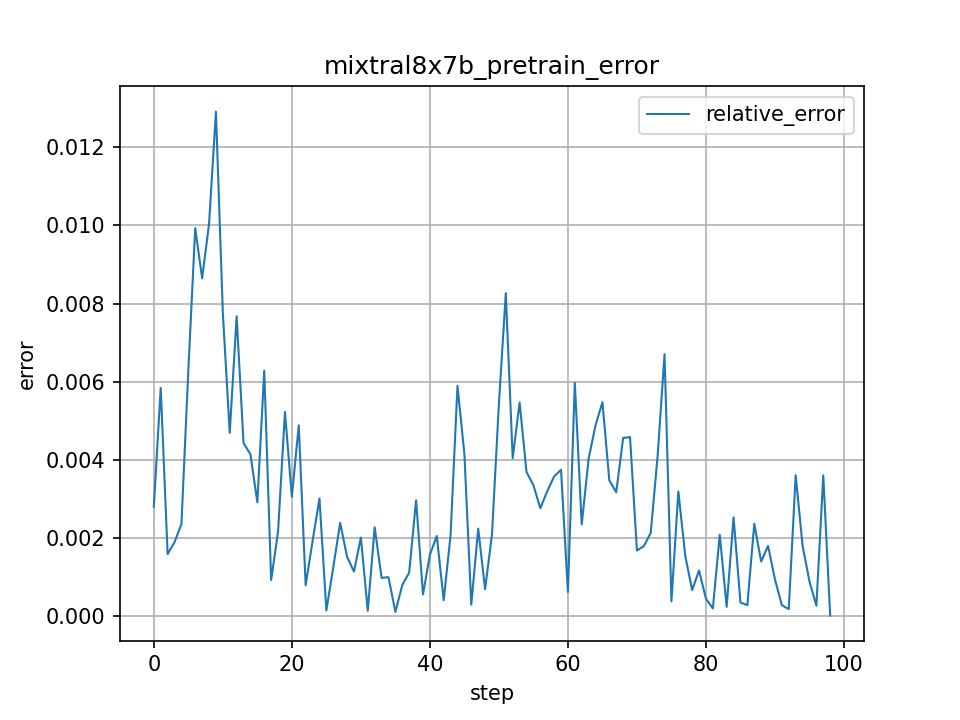
\includegraphics[width=0.6\textwidth]{mlu_gpu_loss_error.png}
    \caption{GPU/MLU loss误差图}
    \label{fig:mlu_gpu_loss_error}
    % \note{注:图注的内容不宜放到图题中。}
\end{figure}



\section{本章小结}
本章首先介绍了  Top-k 算子测试实验所依赖的软硬件环境,紧接着对 
 Top-K算子的测试流程进行了系统的概述。鉴于 Top-k 算子输入参数的多样性和复杂性, 
为了确保测试能够全面覆盖所有参数的取值,基于大/小k两种场景分别进行了功能测试和性能测试。
最后将Top-k算子注册在Pytorch框架中,基于Mixtral8\times7B大语言模型进行Top-k算子的集成测试。
验证了本文Top-k算子的可用性。